\section{Design REST Api}
\subsection{Introduction}
\begin{flushleft}
Cette section représente le fonctionnement de l'API REST sous forme d'un diagramme de classes. Ce schéma montre les interactions entre l'API, le serveur et les utilisateurs. Les fonctionnalités implémentées dans le diagramme de classe de l'application sont reprises sous forme de requêtes liées à l'API.
\end{flushleft}

\subsection{Gestion d'un utlisateur}
\begin{flushleft}
Lorsqu'un utilisateur interagit avec l'application lors de sa connexion, une requête entrante est envoyée à l'API avec les informations de connexion (un mail, un mot de passe, un nom et un type\footnote{client ou fournisseur}).
\end{flushleft}

\begin{flushleft}
Une fois l'utilisateur créé, une requête sortante est renvoyée à l'application. Ici, 3 possibilités de requêtes sont fournies : 201 - Created, 401 - Unauthorized, 404 - Not Found. Les requêtes 401 et 404 sont erreurs renvoyant un message et le code de l'erreur. Quant à la requête 201, celle-ci met à jour l'application. Un client authentifié est reconnu avec des attributs comme typeOfConsumption\footnote{Permet de voir les différents moyens de consommation d'un utilisateur} et isAProvider\footnote{Permet à l'API de savoir si c'est un client ou un fournisseur}. Dans certains cas, les requêtes seront soumises à une vérification de paramètres. Le paramètre vérifié est "isAProvider", restreignant l'accès aux utilisateurs client/fournisseur. Dans le cas où la condition n'est pas respectée, la réponse "401 - Unauthorized" sera envoyée.
\end{flushleft}

\subsection{Ajout de données}
\begin{flushleft}
Lors d'une interaction avec l'API, il est possible d'ajouter ou de créer des données grâce à une requête "POST". Celle-ci permet notament la création de contrats, de portefeuilles, de propositons de contrats pour les fournisseur et l'ajout d'une méthode de consommation. Si l'interaction est validée, la requête "200 - OK" est la réponse de l'API pour l'application créeant donc respectivement l'objet demandé.
\end{flushleft}
\newpage
\subsection{Affichage de données}
\begin{flushleft}
Parmi les fonctionnalités disponible pour un utilisateur, la possibilité de voir une liste de certains objets lui appartenant en fait partie. Lors d'une requête "GET", l'API va rechercher tous les éléments demandés, répondant aux caractéristiques et appartenant à l'utilisateur.
\end{flushleft}

\subsection{Modification/Suppression de données}
\begin{flushleft}
Lorsque qu'un utilisateur souhaite supprimer une donnée, celui-ci appelle l'API avec une requête "DELETE" supprimant donc la donnée correspondante. Lors d'une modification à l'aide d'une requête "PUT", l'API demande la modification de la donnée avec la donnée à modifier ainsi que sa modification.
\end{flushleft}

\subsection{Conclusion}
\begin{flushleft}
En conclusion, un utilisateur peut gérer ses données à l'aide de requêtes POST, PUT, GET, DELETE. Celui-ci a certaines permissions d'accès à ces données et l'API gère ce gestionnaire de données à l'aide de classes.
\newpage

\end{flushleft}
\subsection{schéma}
\begin{figure}[h]
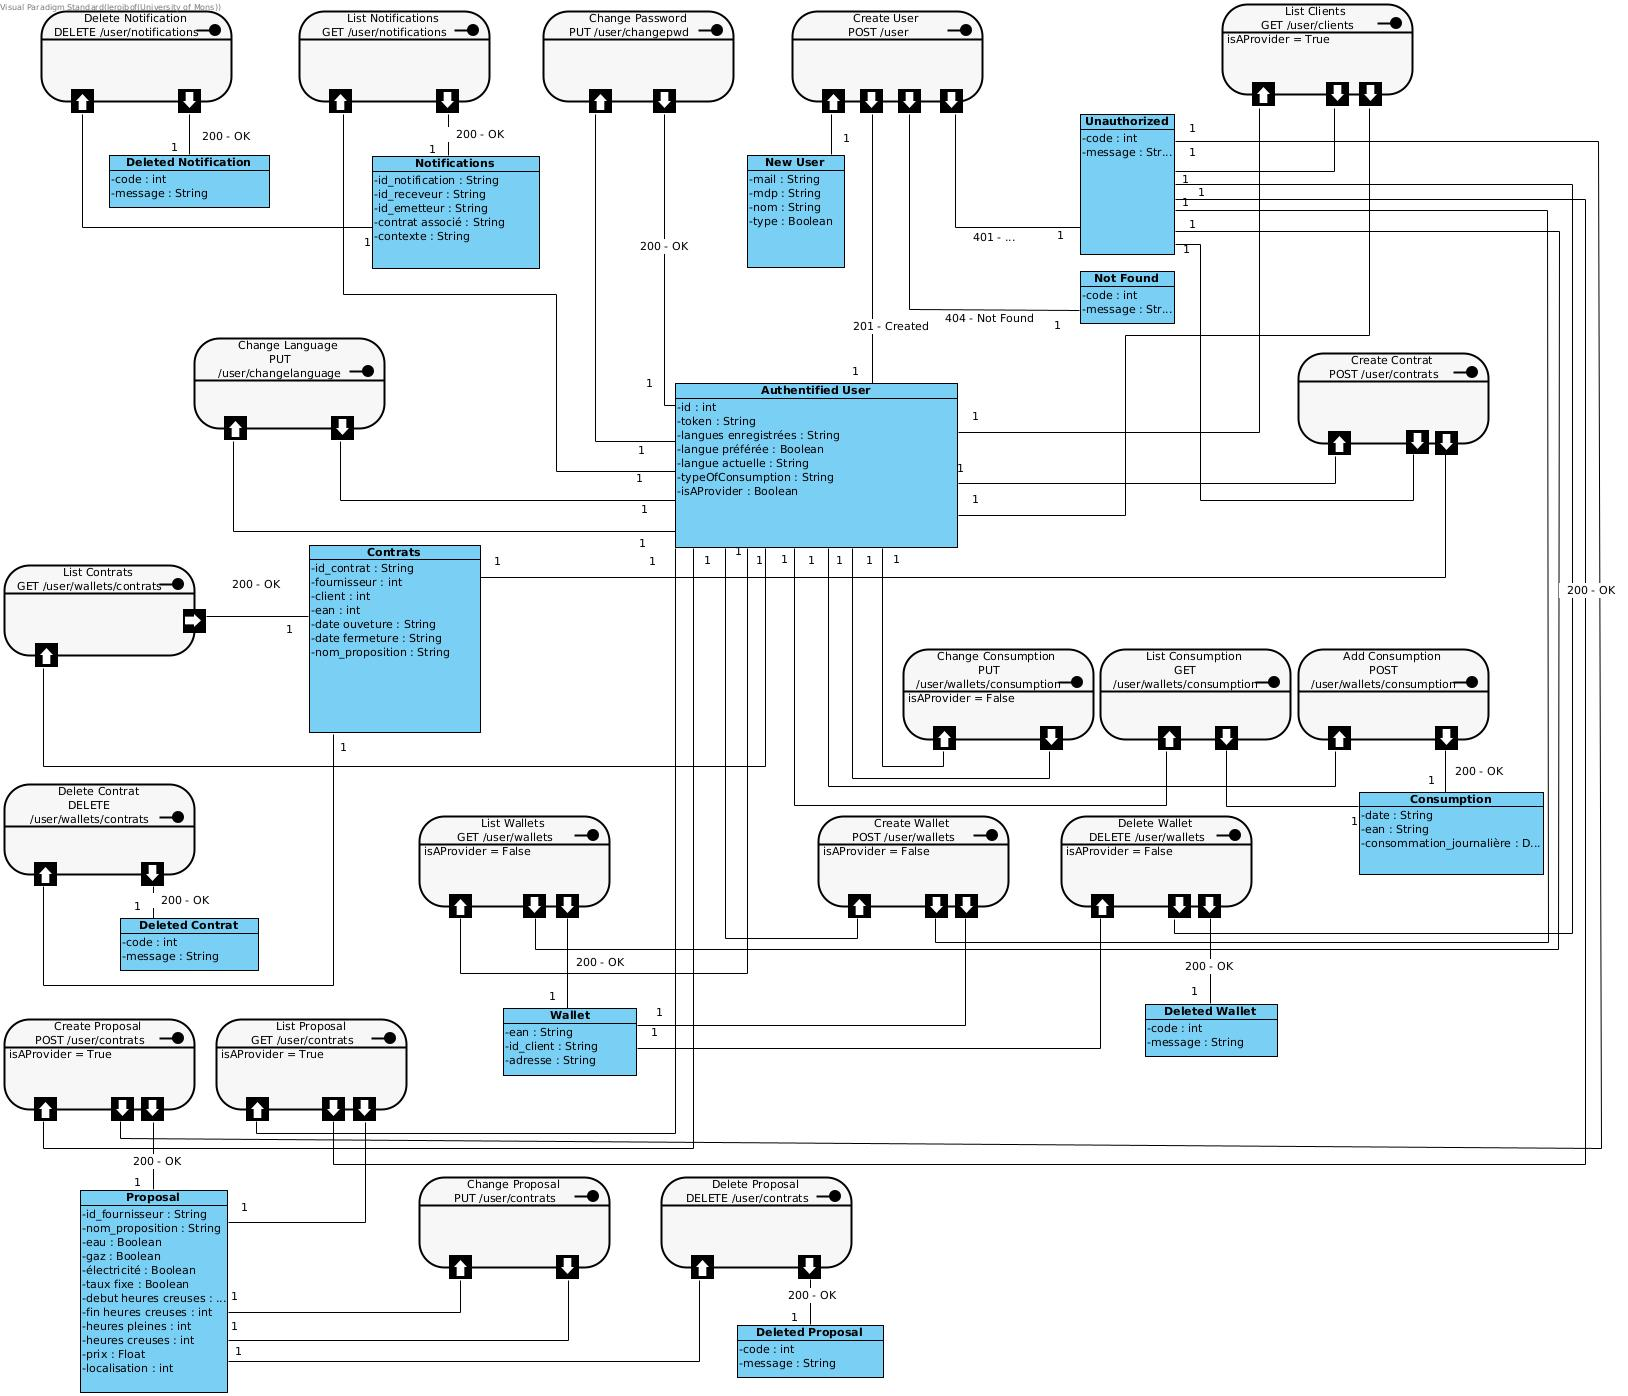
\includegraphics[scale=0.2]{Base/api-rest/img/apirest.jpg}
\end{figure}

